\documentclass{article}

\usepackage{fontspec}
\setmainfont{Open Sans-Regular}
\usepackage{tikz}
\usetikzlibrary{shapes.gates.logic.US}
\input{dft-tikz}
\definecolor{normalfillcolor}{gray}{0.7}
\setlength\paperwidth{30cm}
\setlength\paperheight{50cm}
\setlength\textheight{40cm}
\setlength\hoffset{-1in}
\newdimen\zigzagvert
\zigzagvert=5mm % Connections first go this far down, then zig-zag to
                % their target.
\pagestyle{empty}

\begin{document}
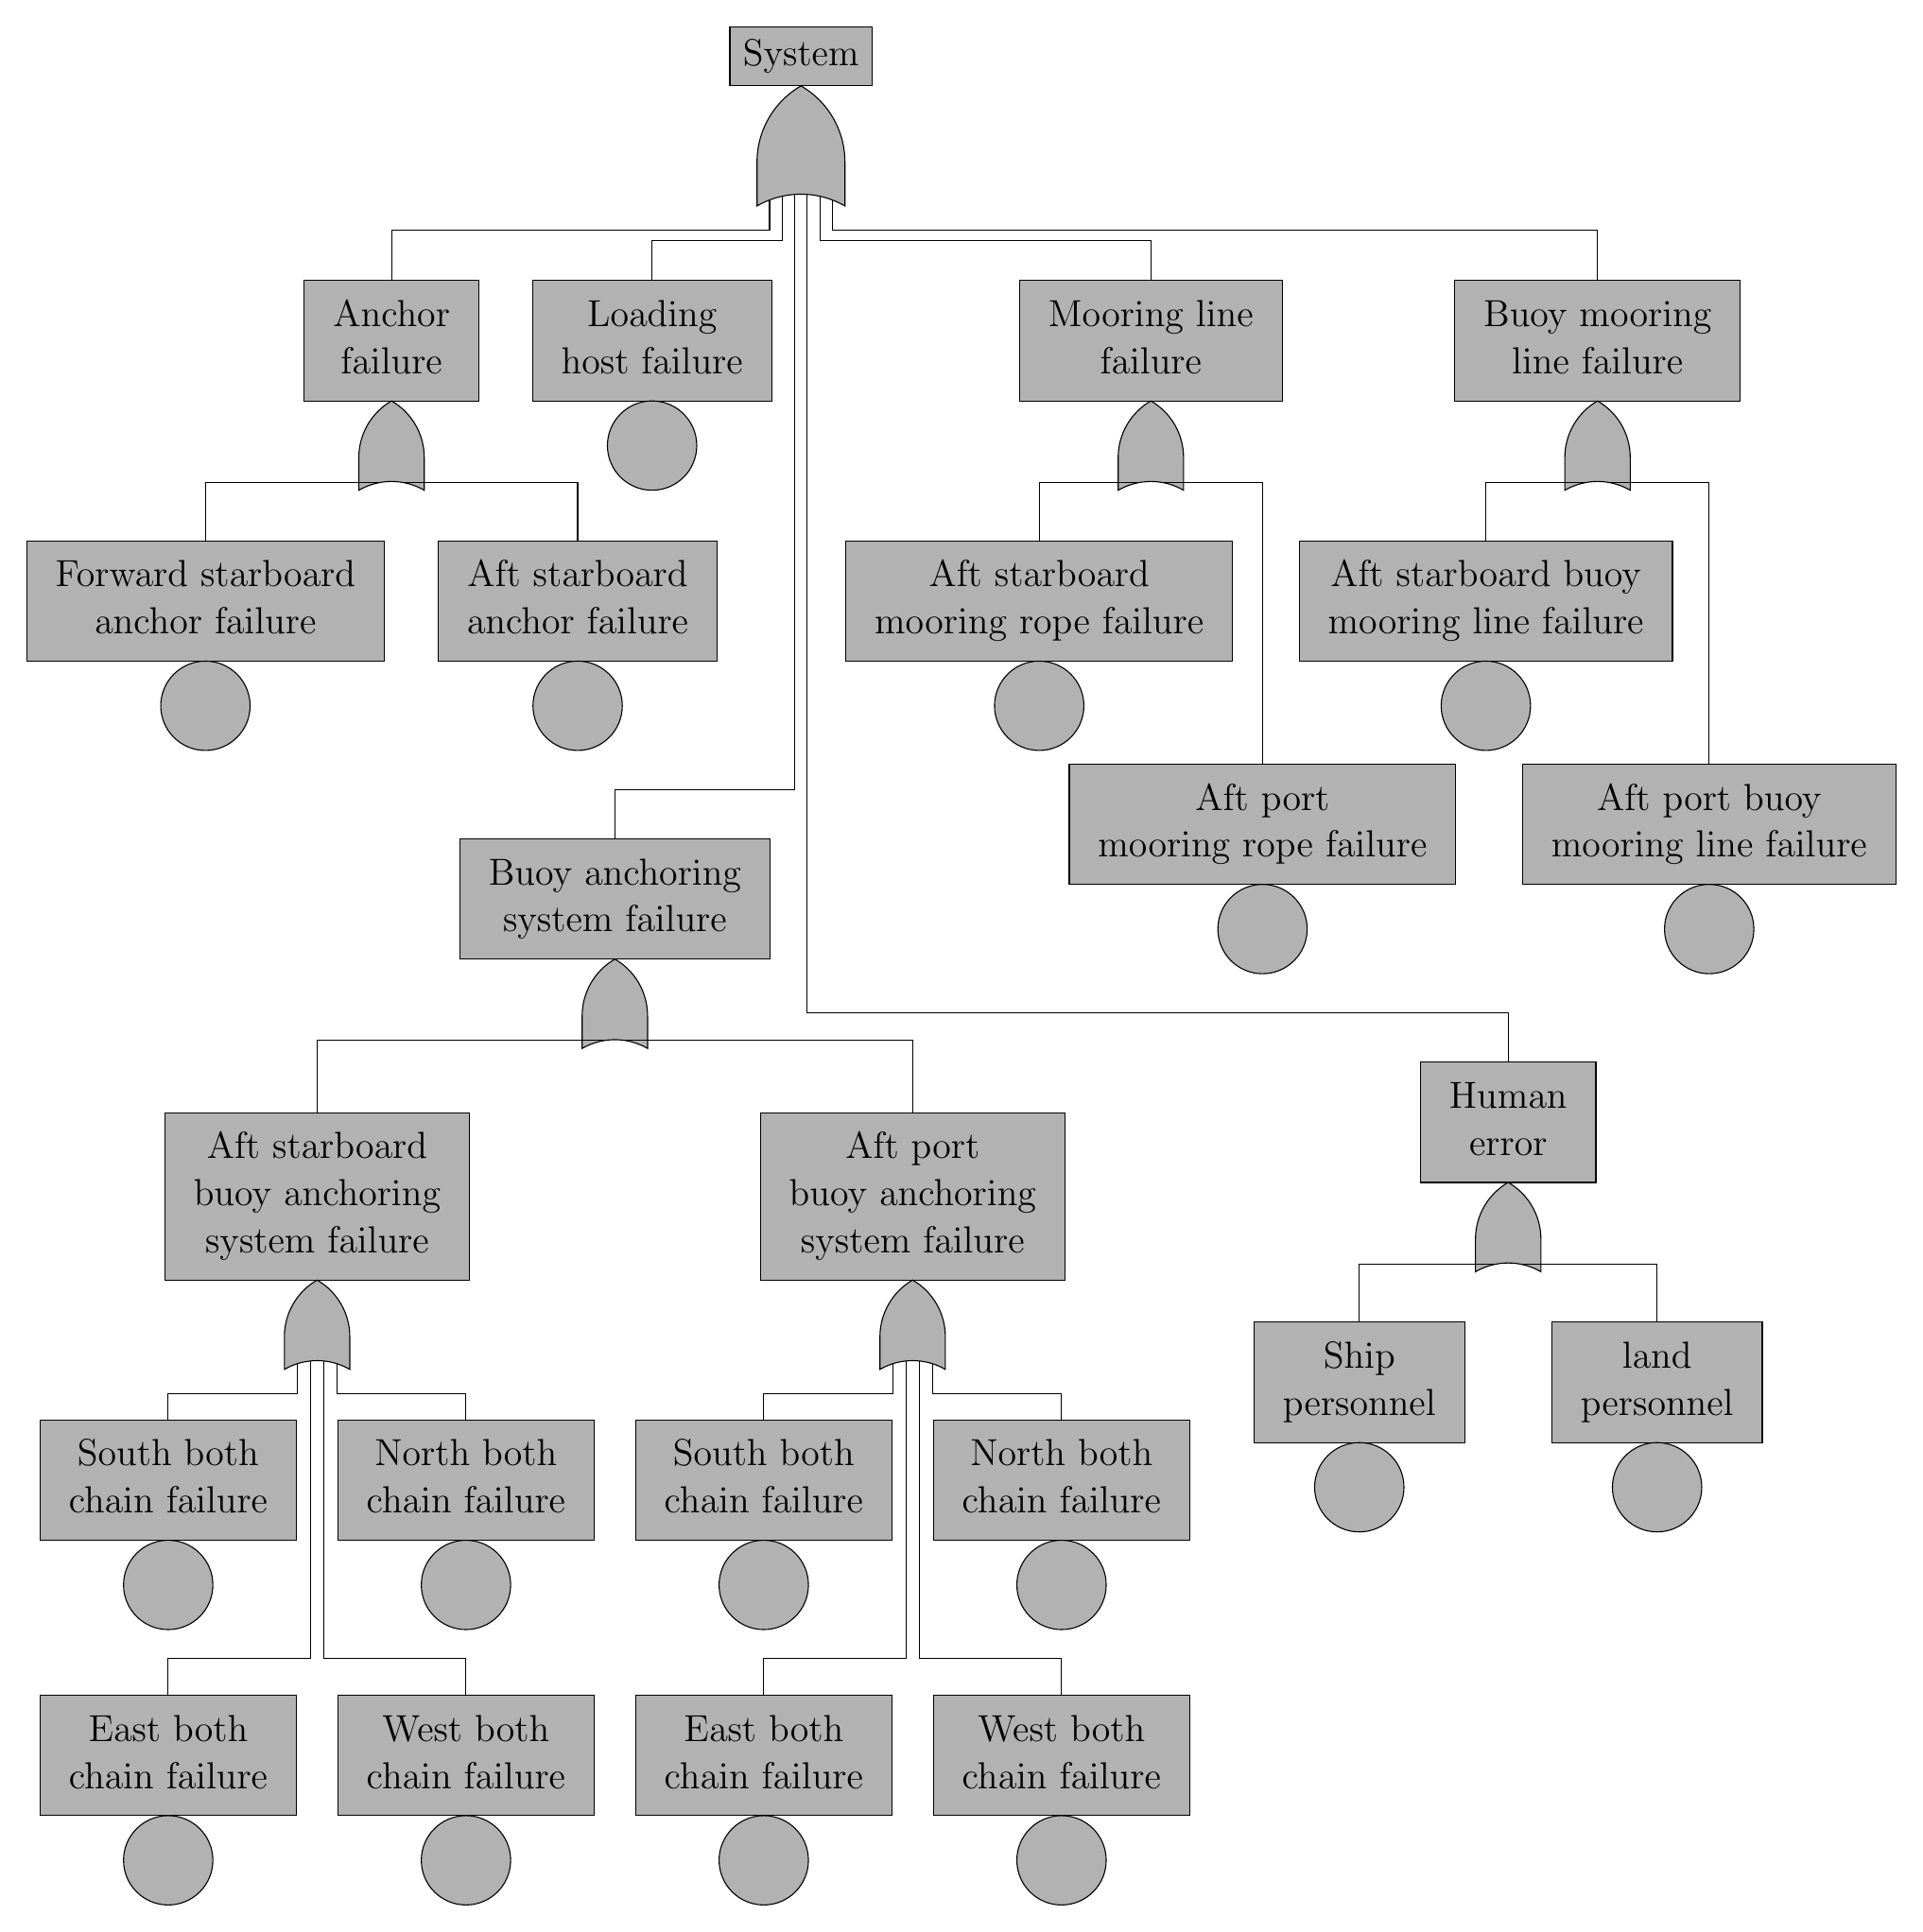
\begin{tikzpicture}[
	rectangle/.style={fill=normalfillcolor, inner sep=5pt},
	node distance=2cm,
	every node/.style={outer sep=0pt,font=\Large},
]
% Input 1 ignored (would be input count).
\def\basicevent#1[#2](#3)#4{
        \node[rectangle, draw, #2, minimum height=5.5mm](#3box){#4};
        \node[circle, minimum width=12mm, fill=normalfillcolor, draw,
		anchor=north] at (#3box.south) (#3) {};
}
% Input 1: Text in triangle.
\def\transferevent#1[#2](#3)#4{
        \node[rectangle, draw, #2, minimum height=5.5mm](#3box){#4};
	\path[draw, fill=normalfillcolor] (#3box.south)
		-- ++(-8mm, -15mm) -- ++(16mm, 0) -- (#3box.south);
	\path (#3box.south) ++ (0, -15mm) node[anchor=south] (#3) {#1};
}
\def\seqevent#1[#2](#3)#4{
        \node[rectangle, draw, #2, minimum height=1cm, minimum width=15mm](#3){};
	\node[anchor=north] at (#3.north) (#3box) {#4};
	\draw[->, line width=1mm] (#3.west) -- (#3.east);
}
\def\orevent#1[#2](#3)#4{
        \node[rectangle, draw, #2, minimum height=5.5mm](#3box){#4};
        \node[or gate US, minimum width=12mm, logic gate inputs=#1, rotate=90, fill=normalfillcolor, draw, anchor=output] at (#3box.south) (#3) {};
}
\def\andevent#1[#2](#3)#4{
        \node[rectangle, draw, #2, minimum height=5.5mm](#3box){#4};
        \node[and gate US, minimum width=12mm, logic gate inputs=#1, rotate=90, fill=normalfillcolor, draw, anchor=output] at (#3box.south) (#3) {};
}
% Input 1: Blank for normal, M for mirrored.
\def\sparegate#1[#2](#3)#4{
        \node[spare#1, fill=normalfillcolor, draw, anchor=north, #2]
		(#3) {};
	\node[anchor=north] at (#3.north) (#3box) {#4};
}
% Input 1 ignored (for consistency).
\def\fdepgate#1[#2](#3)#4{
        \node[fdep, fill=normalfillcolor, draw, anchor=north, #2]
		(#3) {};
	\node[anchor=north] at (#3.north) (#3box) {#4};
}
% \connectZZ{G.input}{vert. distance}{child}.
% Draw a line from G.input down by 'vert. distance', then zig-zag to
% child.
\def\connectcust#1#2#3{
	\draw[-] (#1) -- ++(0,#2) -| (#3box);
}
% \connect{G.input}{child} (Note: Only for vertical connections).
\def\connect#1#2{
	\connectcust{#1}{-\zigzagvert}{#2};
}
	\orevent{nnnnnn}[](top){System}
	\orevent{nn}[below of=top, xshift=-55mm, yshift=-5mm](AF){\begin{tabular}{c}
		Anchor\\failure\end{tabular}}
	\basicevent [below of=top, xshift=-20mm, yshift=-5mm](LHF){\begin{tabular}{c}
		Loading\\host failure\end{tabular}}
	\orevent{nn}[below of=top, xshift=47mm, yshift=-5mm](MLF){\begin{tabular}{c}
		Mooring line\\failure\end{tabular}}
	\orevent{nn}[below of=top, xshift=-25mm,
		yshift=-8cm](BASF){\begin{tabular}{c}Buoy anchoring\\system
		failure\end{tabular}}
	\orevent{nn}[below of=top, xshift=107mm, yshift=-5mm](BMLF){\begin{tabular}{c}
		Buoy mooring\\line failure\end{tabular}}
	\orevent{nn}[below of=top, xshift=95mm, yshift=-11cm](HE)
		{\begin{tabular}{c}Human\\error\end{tabular}}
	\connectcust{top.input 1}{-4mm}{AF}
	\connectcust{top.input 2}{-6mm}{LHF}
	\draw (top.input 3) -- ++(0, -8cm) -| (BASFbox.north);
	\draw (top.input 4) -- ++(0, -11cm) -| (HEbox.north);
	\connectcust{top.input 5}{-6mm}{MLF}
	\connectcust{top.input 6}{-4mm}{BMLF}
	\basicevent [below of=AF, xshift=-25mm](FSA){\begin{tabular}{c}
		Forward starboard\\anchor failure\end{tabular}}
	\basicevent [below of=AF, xshift=25mm](ASA){\begin{tabular}{c}
		Aft starboard\\anchor failure\end{tabular}}
	\connect{AF.input 1}{FSA}
	\connect{AF.input 2}{ASA}
	\basicevent [below of=MLF, xshift=-15mm](SMR){\begin{tabular}{c}
		Aft starboard\\mooring rope failure\end{tabular}}
	\basicevent [below of=MLF, xshift=15mm, yshift=-3cm](PMR){\begin{tabular}{c}
		Aft port\\mooring rope failure\end{tabular}}
	\connect{MLF.input 1}{SMR}
	\connect{MLF.input 2}{PMR}
	\basicevent [below of=BMLF, xshift=-15mm](SMR){\begin{tabular}{c}
		Aft starboard buoy\\mooring line failure\end{tabular}}
	\basicevent [below of=BMLF, xshift=15mm, yshift=-3cm](PMR){\begin{tabular}{c}
		Aft port buoy\\mooring line failure\end{tabular}}
	\connect{BMLF.input 1}{SMR}
	\connect{BMLF.input 2}{PMR}
	\basicevent [below of=HE, xshift=-2cm](SP){\begin{tabular}{c}
		Ship\\personnel\end{tabular}}
	\basicevent [below of=HE, xshift=2cm](LP){\begin{tabular}{c}
		land\\personnel\end{tabular}}
	\connect{HE.input 1}{SP}
	\connect{HE.input 2}{LP}

	\orevent{nnnn}[below of=BASF, xshift=-4cm, yshift=-5mm](STB){\begin{tabular}{c}
		Aft starboard\\buoy anchoring\\system failure\end{tabular}}
	\orevent{nnnn}[below of=BASF, xshift=4cm, yshift=-5mm](PT){\begin{tabular}{c}
		Aft port\\buoy anchoring\\system failure\end{tabular}}
	\connect{BASF.input 1}{STB}
	\connect{BASF.input 2}{PT}

	\basicevent [below of=STB, xshift=-2cm](S){\begin{tabular}{c}
		South both\\chain failure\end{tabular}}
	\basicevent [below of=STB, xshift=2cm](N){\begin{tabular}{c}
		North both\\chain failure\end{tabular}}
	\basicevent [below of=STB, xshift=-2cm, yshift=-37mm](E){\begin{tabular}{c}
		East both\\chain failure\end{tabular}}
	\basicevent [below of=STB, xshift=2cm, yshift=-37mm](W){\begin{tabular}{c}
		West both\\chain failure\end{tabular}}
	\connectcust{STB.input 1}{-4mm}{S}
	\connectcust{STB.input 4}{-4mm}{N}
	\connectcust{STB.input 2}{-4cm}{E}
	\connectcust{STB.input 3}{-4cm}{W}

	\basicevent [below of=PT, xshift=-2cm](S){\begin{tabular}{c}
		South both\\chain failure\end{tabular}}
	\basicevent [below of=PT, xshift=2cm](N){\begin{tabular}{c}
		North both\\chain failure\end{tabular}}
	\basicevent [below of=PT, xshift=-2cm, yshift=-37mm](E){\begin{tabular}{c}
		East both\\chain failure\end{tabular}}
	\basicevent [below of=PT, xshift=2cm, yshift=-37mm](W){\begin{tabular}{c}
		West both\\chain failure\end{tabular}}
	\connectcust{PT.input 1}{-4mm}{S}
	\connectcust{PT.input 4}{-4mm}{N}
	\connectcust{PT.input 2}{-4cm}{E}
	\connectcust{PT.input 3}{-4cm}{W}
\end{tikzpicture}
\end{document}
